\chapter{Conclusions and outlook}\label{chap:conclusions}

In this chapter, we take stock of the current state of the research performed in this work. We begin in Section~\ref{sec:summary} by briefly summarising the key results presented in Chapter~\ref{chap:non-orientable}. We then expand on some avenues of possible further research in Section~\ref{sec:outlook}, speculating on specific lines of inquiry where appropriate. %TODO caveat may not be necessary now

\markedsection{Summary}{Summary of main results}\label{sec:summary}

The central results of this thesis are focused around gaining a deeper understanding of how non-orientability in momentum space alters the topological description of Weyl semimetals---a state of matter that is fundamentally chiral in nature. This was achieved in large part by applying the appropriate tools from algebraic topology to a glide symmetric system featuring a Brillouin zone with $\KS$ topology, of which several salient properties had already been established in Ref.~\cite{Fonseca-Vaidya_nonorientable}.

\subsubsection{Contextualisation of the Poincaré--Hopf theorem}

An important aspect of obtaining a cogent topological description lies in deciding which tools from topology are suitable to use in the first place. To this end, we have placed the role that the Poincaré--Hopf theorem plays in deriving the Nielsen--Ninomiya charge cancellation on firmer theoretical footing. In three dimensions, Poincaré--Hopf states that the singularities of a tangent vector field on a compact manifold should have topological indices which sum to zero. Nielsen--Ninomiya is then usually derived by noting that the $\h(\k)$ appearing in the model Hamiltonian can be considered such a tangent vector field. We note that this is categorically not the case on non-orientable manifolds; in this context, $\h(\k)$ is a section of the trivial $\R^3$-bundle over the manifold, rather than the tangent bundle. The mismatch in orientability between the base manifold and the $\R^3$-bundle is precisely what causes the Poincaré--Hopf/Nielsen--Ninomiya theorems to become modified to a mod 2 charge cancellation.

\subsubsection{Formalism for obtaining twisted coefficients}

In order to obtain a full classification in terms of homology and cohomology on a non-orientable system, one needs to decide how to restore Poincaré duality. This is done by twisting the coefficients of either the homology or the cohomology; only one of these choices yields the correct topological invariants. The correct twisting is usually motivated using arguments relating to vector bundle classification. These arguments are relatively tractable for a free unitary action such as the one featured in the $\KS$ system, but they quickly become conceptually involved when studying more complex symmetries (i.e. those that have fixed points, are anti-unitary, etc.), requiring much mathematical legwork to be done in order to obtain the final topological invariants.

To remedy this situation, we demonstrate that a highly straightforward heuristic arises in the specific context of Weyl semimetals: one can study how a given orientation-reversing symmetry acts on Weyl points. If the symmetric partner of a Weyl point has the same chirality, this indicates a twist in the cohomology, and if it has the opposite chirality, the twist is in the homology. This twist then carries over to the underlying insulating topology, so that this heuristic is also useful for classifying those insulating phases which are mediated by transitional Weyl semimetals. This formalism is not rigorous enough to fully replace vector bundle classification, since in general one still needs to study how any fixed points of the symmetry are treated in the equivariant homology and cohomology. However, these features might also be assessable using similar heuristics, depending on the system. In any case, the formalism is useful for developing physical intuition, and it serves as a good sanity check in classification schemes making use of these twisted groups.

\subsubsection{Classification of $\KS$ bulk and $K^2$ surface invariants}

We provide a full classification and interpretation of the topological invariants on the $\KS$ system arising from a single momentum space glide symmetry, based on the explicitly calculated Mayer--Vietoris sequence in Equation~\eqref{eq:explicit-sequence-nonorientable}. This includes both the insulating invariants, which are classified by $\Z\oplus\Z_2$, and the semimetal invariants, classified by $\Z\oplus\Z_2\oplus\Z^k$ with $k$ the number of Weyl points on $\KS$. Aside from the $\Z_2$ invariant $\nu_z$ which has been well studied previously, we also find a seemingly novel $\Z$ invariant $\nu_x$. We demonstrate how $\nu_x$ and $\nu_z$ can be obtained from the action of the glide symmetry on two of the basic homology invariants in $H_1(\T^3)\cong\Z^3$, and how the third invariant is trivialised by the same action. Based on these observations, we provide two integral equations for explicit calculation of $\nu_x$: Equation~\eqref{eq:z-invariant1} in terms of a simple Chern number in the insulating context, and Equation~\eqref{eq:z-invariant2} in terms of curved planes in the semimetallic context. This illustrates the usefulness of the twisted homology point of view.

We also provide a classification of the surface states arising from truncation in the periodic $S^1$ direction, in the form of the Mayer--Vietoris sequence in Equation~\eqref{eq:K2-MV-explicit}. This sequence has very similar features to the bulk $\KS$ sequence, save for the fact that the $\Z_2$ invariant $\nu_z$ is projected out.

\subsubsection{Clarification of mod 2 charge cancellation}

The Mayer--Vietoris sequence in Equation~\eqref{eq:explicit-sequence-nonorientable} also provides a more solid conceptual basis for the mod 2 charge cancellation on $\KS$ described in Ref.~\cite{Fonseca-Vaidya_nonorientable}. It relates to the fact that the charges of all Weyl points must sum to zero in the group $H^2(\KS)\cong\Z_2$, which appears where a $\Z$ group would usually be in the orientable case. This is closely related to the lack of a canonical orientation at each Weyl point. In particular, it follows that the total chirality is ill defined as an integer, being sensitive to arbitrary local choices of orientation (or equivalently, choice of a fundamental domain). We assert that this amounts to an unphysical degree of freedom, so that any apparent net non-zero chirality cannot have phenomenological consequences.

\subsubsection{Classification of non-orientable Brillouin zones}

Through use of the theory of space groups, we ascertain that there are exactly three other symmetry groups in three dimensions besides the single glide symmetry which have a free action giving rise to a non-orientable fundamental Brillouin zone: $Cc$, $Pca2_1$ and $Pna2_1$. Just as for $\KS$, we provide explicitly calculated Mayer--Vietoris sequences for each of these three systems. Each of them features the same $\Z_2$ charge cancellation as $\KS$; the differences lie in the insulating invariants. Explicitly, the insulating phases under $Cc$ symmetry are classified by $\Z\oplus\Z_2^2$, those under $Pca2_1$ are given by $\Z_2^2$ and those under $Pna2_1$ are given by $\Z_4$. This latter group is especially interesting, featuring a topological invariant of order four.

{\color{blue}\subsubsection{Ansatz for inversion symmetry invariants}}

%TODO Inversion


\markedsection{Recommendations}{Research recommendations}\label{sec:outlook}

%TODO Outlook

{\color{blue}
Outlook points:	

\begin{itemize}	
	\item $\KS$ surface states in $k_x$ and $k_y$ directions
	
	\item The same MV sequence in Equation~\eqref{eq:K2-MV-explicit} may also apply to 2D type AIII Klein bottle WSM with chiral symmetry; there is a difference in Fermi arcs vs. Dirac strings etc. but the topology should be similar.
	
	\item 2D non-Hermitian systems: König, Yang et al. $\to$ Stålhammar \& Rødland $\to$ present work
	
	\item Heuristic approach to dealing with fixed points in equivariant homology may be feasible
	
	\item Applicability of this description is probably limited under addition of non-trivial additional bands, e.g. 4-band models incorporating spin and orbital degrees of freedom. The full scope of applicability is somewhat of an open question at this point. (E.g., how well are 2D chiral WSMs described by this homology picture?)
	
	\item Experimental verification in acoustic crystals may be relatively straightforward.
	
	\item Anti-unitary glide symmetry $\implies$ twisted cohomology on $\KS$? %TODO look into anti-unitary space group symm.
\end{itemize}
}

{\color{red}
\section*{Notes}
Concepts explored in early personal notes:
\begin{itemize}
	\item Calculations of (co)homology and semimetal MV sequence for manifolds in $\geq2$ dimensions:
	\begin{itemize}
		\item All compact surfaces without boundary, i.e.\ the surfaces $M_g$ and $N_g$
		
		\item All spaces of the form $M = K^2 \times \T^{d-2}$
	\end{itemize}
	
	\item $\Sigma$ and the other maps in the MV sequence are difficult to interpret in the $\chi\neq 0$ case (maybe even generally for odd dimensions). Taking the oriented case as an example, the MV sequence ends as
	\begin{align*}
		H^{d-1}(M\setminus\Delta)\ \rightarrow\ H^{d-1}\left(\bigsqcup_{k}S^{d-1}\right) \cong \Z^k\ \overset{\Sigma}{\rightarrow}\ H^d(M) \cong \Z
	\end{align*}
	so that the ``charge configuration'' in $\Z^k$ must map to 0 by $\Sigma$ in order to descend from the semimetal, regardless of whether $\chi=0$.
	
	\item This may imply that the Bloch vector field carries more topological information about the total charge than the MV sequence (which makes sense since it generates \emph{all} homology groups of the valence bundle, and all Betti numbers factor into $\chi$). As a concrete example, consider $M=S^2$ with a single puncture of charge $+2$. The punctured sphere is topologically a disc, so that the valence bundle must be trivial, while the Bloch vector field is topologically non-trivial in the sense that it has an index $+2$ singularity. In addition, all relevant $H_n(A)\oplus H_n(B)$ are zero, so that the semimetal MV reduces to the statement that $H_2(S^2)\cong H_1(S^1)$.
	
	\item It may even be the case that the valence bundle cannot be generated from the Bloch vector field in the $d=2$ case; it's probably worth studying the $d\in\set{3,4,5}$ cases (pullback of some universal bundle) to learn more about this. The $d=3$ case should be especially helpful in understanding how the valence bundle arises from the vector field.
	
	\item The map $H: \R^3\to\la[su](2),\ \vec{h}\mapsto \vec{h}\cdot\vec{\sigma}$ is an isomorphism of Lie algebras, with the cross product as a Lie bracket on $\R^3$. Still the vector field is discontinuous on a non-orientable manifold, while $H$ is not. This suggests an alternative approach for constructing the valence bundle: consider $h$ as a map $M\to\R^d$ instead of an element of $\vct(M)$, and then pull back the universal bundle along the unit map $\hat{h}:M\setminus\Delta\to S^{d-1}$. That is, we detach $\vec{h}$ from the tangent bundle and consider it a more abstract map. An added ``benefit'' of this is that we lose all coordinate dependence. However, this may also be a downside in the sense that the map will not be subject to the same constraints (Poincaré--Hopf etc.) that the vector field is; for example, $S^2\to\R^2,\ x\mapsto(1,0)$ is a perfectly valid map that would violate the hairy ball theorem as a vector field (and this is a result of being unable to cover $S^2$ by a single chart). At this point the question may become more about which description is more physical in nature, and the non-orientable Weyl point paper\cite{Fonseca-Vaidya_nonorientable} seems to imply there may be more to the $h:M\to\R^3$ story. It also seems to agree better with the intuition of an applied external potential removing all Weyl nodes -- something that's impossible for $\chi\neq0$ if charge corresponds to vector field index. It also explains how the valence bundle can be trivial on the once punctured $S^2$.
	
	\item Any smooth $d$-manifold can be given a CW complex structure with one $d$-cell (\href{https://mathoverflow.net/questions/120799/manifolds-admitting-cw-structure-with-single-n-cell}{link}). On this $d$-cell there is an exact correspondence between vector fields and maps to $\R^d$, since it can be embedded in $\R^d$. What distinguishes the two is how points on the boundary of the $d$-cell are identified with each other; this determines whether the ``vectors'' need to change orientation. To illustrate:\\
	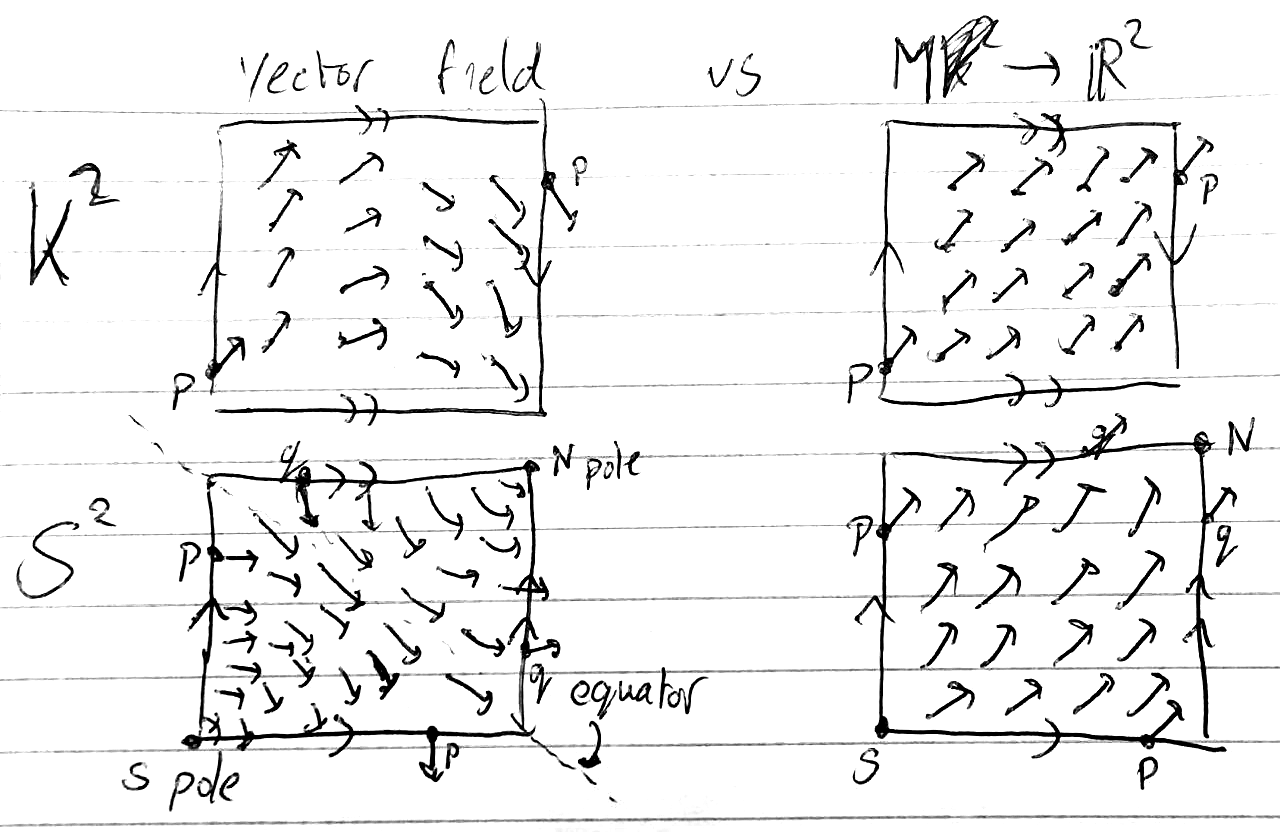
\includegraphics[width=.9\textwidth]{Images/vectorfield-vs-map}
	
	\item On any orientable manifold, the Stokes' theorem argument shows that the total charge must be zero regardless of Euler characteristic:
	\[
	\sum_{\alpha}w(S_\alpha) = \sum_{\alpha}\int_{S_\alpha} c_1(E) = \sum_{\alpha}\int_{S_\alpha}\frac{\Tr\Fc}{2\pi} = \int_{B'} \dd{\frac{\Tr\Fc}{2\pi}} = 0
	\]
	where the last equality holds by the Bianchi identity for the trace. This means the valence bundle cannot be a pullback along a tangent vector field for $\chi\neq0$.
	
	On a non-orientable manifold, this argument doesn't hold since the integral over $B'$ isn't well defined.
\end{itemize}
}  % end red colour